% Copia que genera armar.py desde resultados.tex de la carpeta de su sección; los cambios se hacen allí y se vuelve a armar.
% Sección de resultados del proyecto (Entregables 1 a 3). Se incluye desde main.tex. Toda cifra del texto, de las
% tablas y de las figuras la produce generar.py a partir de los resultados guardados del Entregable 3 (datos/*.csv).
\section{Resultados}
\label{sec:resultados}

Cada cifra de esta sección la reproduce un único guion, \texttt{generar.py}, desde los resultados guardados
del Entregable 3; guion, datos y figuras acompañan al código del proyecto en
\url{https://github.com/RubenEsg/Prediccion-de-fuga-de-clientes-en-fintech}.

\subsection{Resumen del montaje experimental}
\label{sec:montaje}

Los datos son los 48.723 clientes de COFINFAD \citep{cofinfad2025} con 48 predictores ($p = 78$ columnas),
partidos 80/20 con la semilla 42. En clasificación la etiqueta de riesgo alto es el cuarto
superior de \cp\ ($\tau = 0{,}3927$; 24,6~\% de positivos en la prueba). Cada modelo entra con su mejor
combinación según el bucle externo de la validación anidada $5 \times 3$ (mismos pliegues) y toca la prueba una
sola vez. La métrica principal es el AUC en clasificación y el RMSE en regresión; las secundarias, el AUC-PR, el
F1, el MCC y la exactitud balanceada con el 25~\% de capacidad de campaña, el ECE recalibrado, el MAE, el MAPE y
el $R^2$. El protocolo fija $\alpha = 0{,}05$ y Holm \citep{holm1979} sobre las siete comparaciones de cada
prueba. La métrica principal, $\alpha$, Holm, DeLong, Diebold-Mariano y el \emph{Model Confidence Set} se
fijaron en el Entregable 3 antes de evaluar la prueba; la $t$ corregida, McNemar, la bayesiana (con regiones de
equivalencia de $\pm 0{,}01$ de AUC y $\pm 0{,}0005$ de RMSE fijadas antes de ejecutarla) y los análisis de
sensibilidad son posteriores y exploratorios.

\subsection{Desempeño predictivo global}
\label{sec:global}

\paragraph{Clasificación.}
La tabla~\ref{tab:clasificacion} resume la prueba y la figura~\ref{fig:folds} los pliegues. En la prueba la EBM
obtiene el mayor AUC de los ocho modelos, 0,8289 con intervalo BCa [0,8206; 0,8366], seguida de XGBoost,
Random Forest y el árbol de decisión (0,8283 a 0,8243); después vienen k-NN (0,787), los lineales (0,771) y
Naive Bayes (0,666). En la validación anidada la EBM queda cuarta, a 0,0040 de XGBoost y del árbol, el orden
de la desviación entre pliegues. La misma estructura de tres grupos aparece en el AUC-PR (0,551) y en las
curvas ROC y precisión-\emph{recall} de la
figura~\ref{fig:roc_pr}. En el
punto de operación, en cambio, los siete modelos distintos de Naive Bayes son indistinguibles: contactando al
25~\% de mayor riesgo, la EBM captura el 51,2~\% de la fuga con una precisión del 50,4~\% (MCC 0,346) y la
regresión logística el 51,1~\% (MCC 0,344); la tabla~\ref{tab:confusion} da las matrices de confusión con esa
regla y con el umbral 0,5. Las probabilidades sin
recalibrar están sesgadas en los modelos con ponderación (ECE de 0,170 en la EBM); la recalibración isotónica
ajustada con predicciones fuera de pliegue lo deja entre 0,003 y 0,010 y apenas mueve el AUC
(figura~\ref{fig:calibration}). En resumen, por el valor puntual del AUC de prueba y del AUC-PR la EBM queda
por delante de las siete referencias, aunque solo cuatro ventajas son significativas
(sección~\ref{sec:pruebas}); la mayor es $+0{,}058$ de AUC frente a la logística ($+7{,}5$~\% relativo) y la
menor, $+0{,}0006$ frente a XGBoost; por el AUC externo gana cuatro y pierde tres, y en el punto de operación
empata con seis.

\paragraph{Regresión.}
Según la tabla~\ref{tab:regresion}, XGBoost tiene el menor RMSE de prueba (0,05917) y la EBM el segundo
(0,05925), con Random Forest y el árbol dentro de los mismos intervalos; los lineales quedan un 4~\% por encima
y k-NN un 7~\%. El $R^2$ pasa de 0,151 en Ridge y Lasso a 0,216 en la EBM y 0,218 en XGBoost, y el MAPE, de
17,1 a 16,0~\%: la EBM pierde con XGBoost en las cuatro métricas por milésimas o menos y gana a los otros seis.
El pronóstico sigue la tendencia pero
se comprime hacia la media (figura~\ref{fig:regression}), y el residuo de la EBM es asimétrico (asimetría
$-0{,}90$) y no normal, sin heterocedasticidad (White, $p = 0{,}67$) ni dependencia en el orden del archivo
(Ljung-Box, $p = 0{,}81$), según el diagnóstico del Entregable 3; la causa se identifica en la
sección~\ref{sec:errores}.

\paragraph{Frente a la entrega anterior.}
En su partición y etiqueta de la mediana (tabla~\ref{tab:entrega2}), la EBM sube el AUC de la logística L1 de
0,6832 a 0,7187 y baja el RMSE del Lasso de 0,06166 a 0,05926 ($p$ ajustado $< 0{,}001$ en DeLong y en
Diebold-Mariano); frente a XGBoost queda a $-0{,}0019$ de AUC ($p = 0{,}20$) y a $0{,}00007$ de RMSE
($p = 0{,}07$).

\begin{table}[tbp]
  \centering\scriptsize\setlength{\tabcolsep}{3pt}
  \caption{Clasificación (riesgo alto = percentil 75): mejor combinación de cada modelo según el bucle externo. AUC externa (media $\pm$ desviación de los 5 pliegues), AUC de prueba con intervalo \emph{bootstrap} BCa al 95~\%, AUC-PR y, en el punto de operación que contacta al 25~\% de mayor riesgo, F1, MCC y exactitud balanceada; ECE tras la recalibración isotónica. Las métricas secundarias son valores puntuales de la prueba; el \emph{recall} y la precisión de ese punto están en la tabla~\ref{tab:confusion}. Negrita: mejor; subrayado: segundo (los empates comparten la marca). $^{\dagger}$: difiere de la EBM en DeLong tras Holm; $^{\ddagger}$: en la $t$ corregida tras Holm.}
  \label{tab:clasificacion}
  \begin{tabular}{@{}l c c c c c c c@{}}
    \toprule
    Modelo & AUC externa & AUC prueba [IC 95~\%] & AUC-PR & F1$_{25}$ & MCC$_{25}$ & Ex. bal.$_{25}$ & ECE \\
    \midrule
    \textbf{EBM (propuesto)} & $0{,}8292$ $\pm$ $0{,}0037$ & {\boldmath\textbf{$0{,}8289$ [$0{,}8206$; $0{,}8366$]}} & {\boldmath\textbf{$0{,}551$}} & {\boldmath\textbf{$0{,}508$}} & {\boldmath\textbf{$0{,}346$}} & {\boldmath\textbf{$0{,}674$}} & $0{,}006$ \\
    XGBoost & {\boldmath\textbf{$0{,}8332$ $\pm$ $0{,}0049$}} & \underline{$0{,}8283$ [$0{,}8203$; $0{,}8359$]} & \underline{$0{,}548$} & $0{,}506$ & $0{,}343$ & \underline{$0{,}673$} & $0{,}007$ \\
    Random Forest & \underline{$0{,}8326$ $\pm$ $0{,}0029$} & $0{,}8260$ [$0{,}8184$; $0{,}8338$] & $0{,}544$ & $0{,}490$ & $0{,}321$ & $0{,}662$ & {\boldmath\textbf{$0{,}003$}} \\
    Árbol de decisión & {\boldmath\textbf{$0{,}8332$ $\pm$ $0{,}0021$}} & $0{,}8243$ [$0{,}8165$; $0{,}8319$] & $0{,}530$ & $0{,}498$ & $0{,}333$ & $0{,}667$ & $0{,}010$ \\
    k-NN$^{\dagger\ddagger}$ & $0{,}7836$ $\pm$ $0{,}0072$ & $0{,}7874$ [$0{,}7777$; $0{,}7966$] & $0{,}502$ & $0{,}504$ & $0{,}341$ & $0{,}671$ & $0{,}008$ \\
    Regresión logística$^{\dagger\ddagger}$ & $0{,}7644$ $\pm$ $0{,}0047$ & $0{,}7709$ [$0{,}7600$; $0{,}7806$] & $0{,}508$ & \underline{$0{,}507$} & \underline{$0{,}344$} & \underline{$0{,}673$} & $0{,}006$ \\
    SVM lineal$^{\dagger\ddagger}$ & $0{,}7641$ $\pm$ $0{,}0044$ & $0{,}7706$ [$0{,}7599$; $0{,}7803$] & $0{,}507$ & \underline{$0{,}507$} & \underline{$0{,}344$} & \underline{$0{,}673$} & $0{,}007$ \\
    Naive Bayes$^{\dagger\ddagger}$ & $0{,}6722$ $\pm$ $0{,}0119$ & $0{,}6662$ [$0{,}6537$; $0{,}6787$] & $0{,}363$ & $0{,}405$ & $0{,}209$ & $0{,}605$ & \underline{$0{,}004$} \\
    \bottomrule
  \end{tabular}
\end{table}

\begin{table}[tbp]
  \centering\small\setlength{\tabcolsep}{3pt}
  \caption{Matrices de confusión en la prueba (9.745 clientes, 2.399 de riesgo alto) de la EBM y de XGBoost con la regla de decisión de la campaña (se contacta al 25~\% de mayor puntaje, 2.436 clientes) y con el umbral 0,5 de probabilidad: verdaderos positivos (VP), falsos positivos (FP), falsos negativos (FN), verdaderos negativos (VN), precisión y \emph{recall}.}
  \label{tab:confusion}
  \begin{tabular}{@{}l l r r r r c c@{}}
    \toprule
    Regla & Modelo & VP & FP & FN & VN & Precisión & Recall \\
    \midrule
    25~\% de mayor riesgo & \textbf{EBM (propuesto)} & 1.228 & 1.208 & 1.171 & 6.138 & $0{,}504$ & $0{,}512$ \\
    25~\% de mayor riesgo & XGBoost & 1.224 & 1.212 & 1.175 & 6.134 & $0{,}502$ & $0{,}510$ \\
    \midrule
    umbral 0,5 & \textbf{EBM (propuesto)} & 1.697 & 1.928 & 702 & 5.418 & $0{,}468$ & $0{,}707$ \\
    umbral 0,5 & XGBoost & 2.395 & 2.956 & 4 & 4.390 & $0{,}448$ & $0{,}998$ \\
    \bottomrule
  \end{tabular}
\end{table}

\begin{table}[tbp]
  \centering\scriptsize\setlength{\tabcolsep}{1.5pt}
  \caption{Regresión de \cp: mejor optimizador de cada modelo según el bucle externo. RMSE externo (media $\pm$ desviación de los 5 pliegues), RMSE de prueba con intervalo BCa al 95~\%, MAE, MAPE y $R^2$ con intervalo BCa, y $p$-valor del \emph{Model Confidence Set} al 90~\% (pertenecen al conjunto los modelos con $p > 0{,}10$). Negrita: mejor; subrayado: segundo. $^{\dagger}$: difiere de la EBM en Diebold-Mariano tras Holm; $^{\ddagger}$: en la $t$ corregida tras Holm.}
  \label{tab:regresion}
  \begin{tabular}{@{}l c c c c c c@{}}
    \toprule
    Modelo & RMSE externo & RMSE prueba [IC 95~\%] & MAE & MAPE & $R^2$ [IC 95~\%] & $p$ MCS \\
    \midrule
    XGBoost & {\boldmath\textbf{$0{,}05898$ $\pm$ $0{,}00040$}} & {\boldmath\textbf{$0{,}05917$ [$0{,}05841$; $0{,}06002$]}} & {\boldmath\textbf{$0{,}0471$}} & {\boldmath\textbf{$15{,}98$~\%}} & {\boldmath\textbf{$0{,}218$ [$0{,}203$; $0{,}232$]}} & $1{,}000$ \\
    \textbf{EBM (propuesto)} & \underline{$0{,}05903$ $\pm$ $0{,}00043$} & \underline{$0{,}05925$ [$0{,}05849$; $0{,}06009$]} & \underline{$0{,}0472$} & \underline{$16{,}03$~\%} & \underline{$0{,}216$ [$0{,}201$; $0{,}230$]} & $0{,}072$ \\
    Random Forest & $0{,}05915$ $\pm$ $0{,}00039$ & $0{,}05931$ [$0{,}05854$; $0{,}06013$] & $0{,}0473$ & $16{,}05$~\% & $0{,}215$ [$0{,}200$; $0{,}228$] & $0{,}006$ \\
    Árbol de decisión & $0{,}05926$ $\pm$ $0{,}00038$ & $0{,}05944$ [$0{,}05864$; $0{,}06025$] & $0{,}0475$ & $16{,}11$~\% & $0{,}211$ [$0{,}196$; $0{,}225$] & $<0{,}001$ \\
    Lasso$^{\dagger\ddagger}$ & $0{,}06180$ $\pm$ $0{,}00048$ & $0{,}06166$ [$0{,}06082$; $0{,}06251$] & $0{,}0507$ & $17{,}10$~\% & $0{,}151$ [$0{,}138$; $0{,}164$] & $<0{,}001$ \\
    Ridge$^{\dagger\ddagger}$ & $0{,}06182$ $\pm$ $0{,}00048$ & $0{,}06167$ [$0{,}06082$; $0{,}06252$] & $0{,}0507$ & $17{,}10$~\% & $0{,}151$ [$0{,}138$; $0{,}164$] & $<0{,}001$ \\
    SVR lineal$^{\dagger\ddagger}$ & $0{,}06183$ $\pm$ $0{,}00047$ & $0{,}06170$ [$0{,}06087$; $0{,}06255$] & $0{,}0507$ & $17{,}10$~\% & $0{,}150$ [$0{,}137$; $0{,}163$] & $<0{,}001$ \\
    k-NN$^{\dagger\ddagger}$ & $0{,}06335$ $\pm$ $0{,}00042$ & $0{,}06321$ [$0{,}06238$; $0{,}06409$] & $0{,}0511$ & $17{,}28$~\% & $0{,}108$ [$0{,}101$; $0{,}115$] & $<0{,}001$ \\
    \bottomrule
  \end{tabular}
\end{table}

\begin{table}[tbp]
  \centering\scriptsize\setlength{\tabcolsep}{2pt}
  \caption{Comparación con los modelos de la entrega anterior (E2) en su misma partición, etiqueta (mediana estimada con el entrenamiento) y prueba, tal como la calculó el Entregable 3. Clasificación: AUC con intervalo BCa, \emph{recall} con umbral 0,5, mejora de AUC frente a la logística L1 con intervalo BCa, $z$ de DeLong y $p$ ajustado por Holm, delta de Cliff sobre los 5 pliegues. Regresión: RMSE con intervalo BCa, $R^2$, reducción del RMSE frente al Lasso con intervalo BCa, Diebold-Mariano (HLN) y $p$ ajustado, delta de Cliff entre pliegues.}
  \label{tab:entrega2}
  \begin{tabular}{@{}l c c c c c@{}}
    \toprule
    Modelo & AUC o RMSE [IC 95~\%] & Recall$_{0{,}5}$ o $R^2$ & Mejora vs.\ E2 [IC 95~\%] & $z$ o DM; $p$ & $\delta$ \\
    \midrule
    Logística L1 (E2) & $0{,}6832$ [$0{,}6725$; $0{,}6931$] & $0{,}6515$ & -- & -- & -- \\
    XGBoost & $0{,}7206$ [$0{,}7107$; $0{,}7302$] & $0{,}6375$ & $+0{,}0374$ [$0{,}0303$; $0{,}0449$] & $10{,}06$; $2{,}5 \times 10^{-23}$ & $+1{,}00$ \\
    \textbf{EBM (propuesto)} & $0{,}7187$ [$0{,}7084$; $0{,}7284$] & $0{,}6565$ & $+0{,}0355$ [$0{,}0281$; $0{,}0434$] & $9{,}02$; $3{,}8 \times 10^{-19}$ & $+1{,}00$ \\
    \midrule
    Lasso (E2) & $0{,}06166$ [$0{,}06082$; $0{,}06251$] & $0{,}1511$ & -- & -- & -- \\
    XGBoost & $0{,}05919$ [$0{,}05843$; $0{,}06004$] & $0{,}2177$ & $+0{,}00247$ [$0{,}00210$; $0{,}00279$] & $14{,}05$; $5{,}9 \times 10^{-44}$ & $+1{,}00$ \\
    \textbf{EBM (propuesto)} & $0{,}05926$ [$0{,}05849$; $0{,}06010$] & $0{,}2159$ & $+0{,}00240$ [$0{,}00205$; $0{,}00274$] & $13{,}33$; $7{,}1 \times 10^{-40}$ & $+1{,}00$ \\
    \bottomrule
  \end{tabular}
\end{table}


\begin{figure}[tbp]
  \centering
  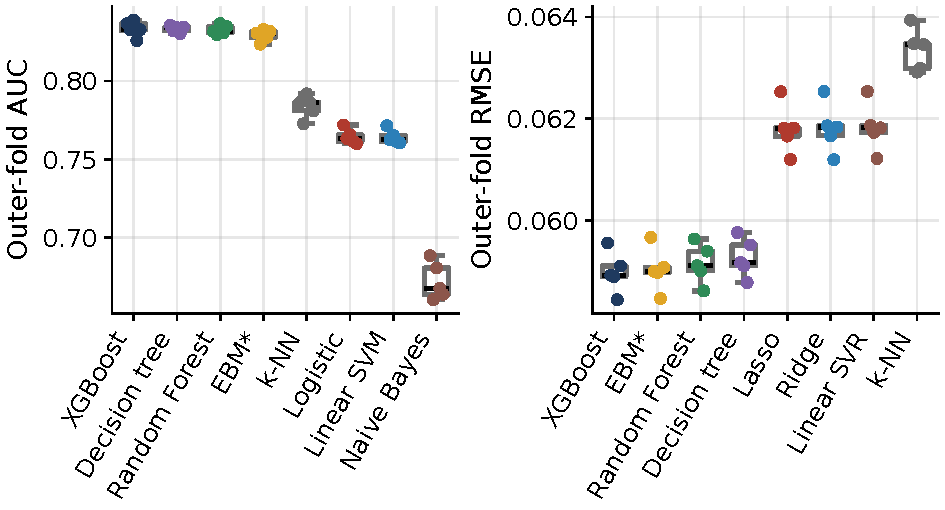
\includegraphics[width=\linewidth]{fig_folds.pdf}
  \caption{Métrica principal en cada uno de los 5 pliegues externos (puntos) y su diagrama de caja (mediana y
  cuartiles; bigotes hasta el mínimo y el máximo) para la mejor combinación de cada modelo: AUC en clasificación
  (izquierda) y RMSE en regresión (derecha). El asterisco marca el modelo propuesto.}
  \label{fig:folds}
\end{figure}

\begin{figure}[tbp]
  \centering
  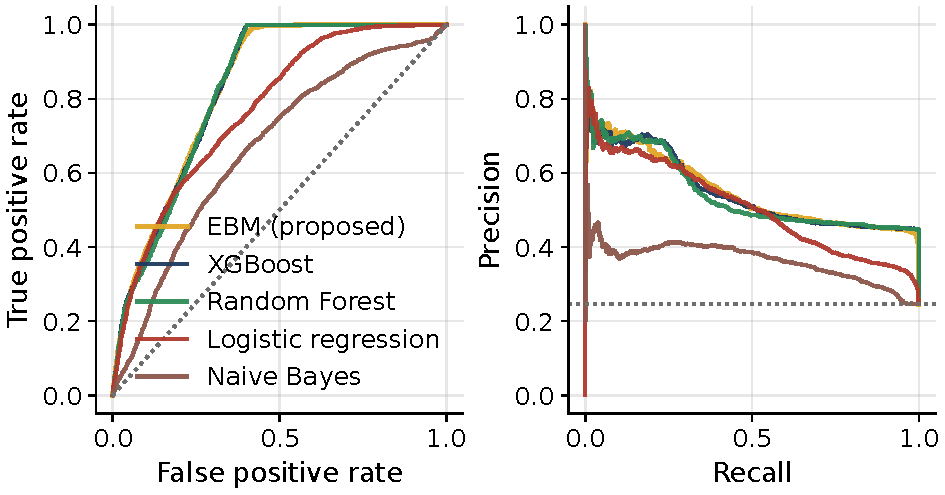
\includegraphics[width=\linewidth]{fig_roc_pr.pdf}
  \caption{Curvas ROC (izquierda) y precisión-\emph{recall} (derecha) en la prueba para la EBM, XGBoost, Random
  Forest, la regresión logística y Naive Bayes; la línea punteada es el azar (en precisión-\emph{recall}, la
  prevalencia de 0,246).}
  \label{fig:roc_pr}
\end{figure}

\begin{figure}[tbp]
  \centering
  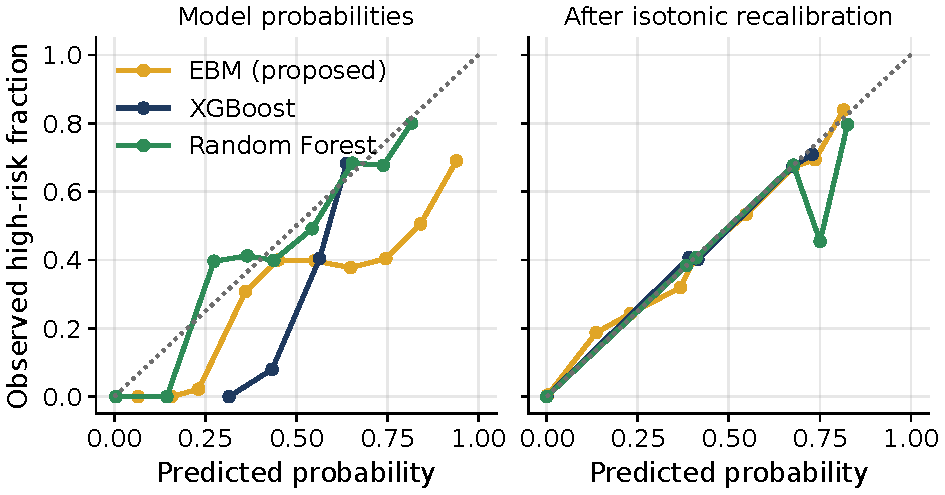
\includegraphics[width=\linewidth]{fig_calibration.pdf}
  \caption{Diagramas de confiabilidad en la prueba (10 intervalos de probabilidad) de la EBM, XGBoost y Random
  Forest antes (izquierda) y después (derecha) de la recalibración isotónica ajustada con predicciones fuera de
  pliegue del entrenamiento; la diagonal punteada es la calibración perfecta.}
  \label{fig:calibration}
\end{figure}

\begin{figure}[tbp]
  \centering
  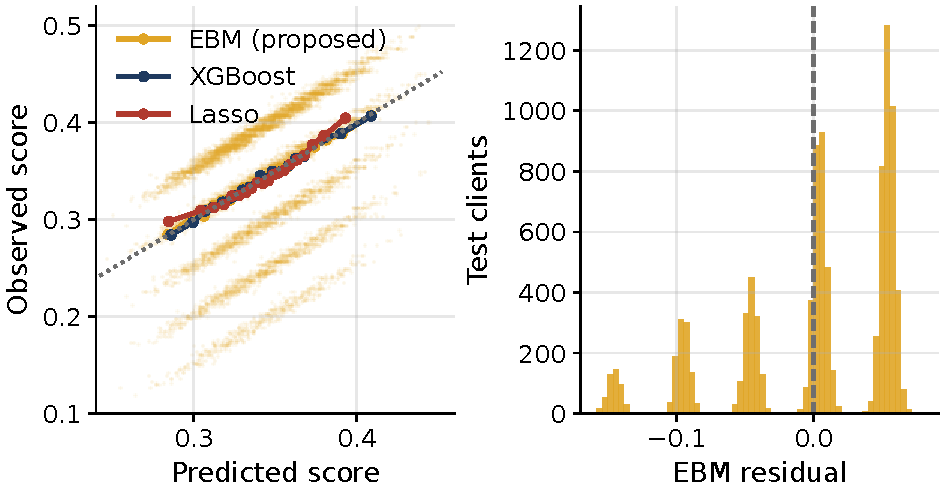
\includegraphics[width=\linewidth]{fig_regression.pdf}
  \caption{Regresión en la prueba. Izquierda: puntaje observado frente al pronóstico de la EBM (puntos,
  un cliente cada uno) y valor observado medio frente al pronóstico medio en 20 grupos de igual tamaño ordenados
  por el pronóstico para la EBM, XGBoost y Lasso (líneas); la diagonal punteada es la calibración perfecta.
  Derecha: distribución del residuo de la EBM (observado $-$ pronóstico).}
  \label{fig:regression}
\end{figure}

\subsection{Resultados de las pruebas de significancia}
\label{sec:pruebas}

Las tablas~\ref{tab:pruebas_clasificacion} a~\ref{tab:efectos_regresion} recogen, para cada modelo de
referencia, las pruebas, la diferencia con la EBM con su intervalo BCa de 2.000 réplicas y los tamaños de
efecto (figura~\ref{fig:intervals}). En
clasificación se aplican la $t$ pareada con varianza corregida de \citet{nadeau2003} sobre los AUC de los
cinco pliegues externos, DeLong \citep{delong1988} sobre la prueba, McNemar exacta \citep{mcnemar1947} sobre
las clases del punto de operación y la $t$ correlacionada bayesiana con región de equivalencia práctica
\citep{corani2015,benavoli2017}; en regresión, la $t$ corregida sobre el RMSE de los pliegues, Diebold-Mariano
con la corrección de \citet{harvey1997} sobre las pérdidas cuadráticas de la prueba, la bayesiana y, como
complemento, el \emph{Model Confidence Set} al 90~\% \citep{hansen2011mcs} con \emph{bootstrap} estacionario
\citep{politis1994}. Con cinco pliegues Wilcoxon no puede rechazar ($p$ mínimo 0,0625); se reporta la delta
de Cliff.

\paragraph{Clasificación.}
Frente a los cuatro modelos sin árboles la evidencia de diferencia es unánime: la $t$ corregida da
estadísticos de 14,3 a 23,2 y DeLong de 12,5 a 27,8, todos con $p$ ajustado menor que 0,001; los intervalos
de $\Delta$AUC quedan lejos de cero (de $+0{,}042$ a $+0{,}163$); la probabilidad posterior de que la EBM sea
mejor es mayor que 0,999, y el delta de Cliff es $+1$: la EBM gana en los cinco pliegues. Frente a XGBoost,
Random Forest y el árbol ninguna prueba rechaza: la $t$ corregida ($p$ ajustado de 0,16 a 0,25), DeLong ($p$
ajustado de 0,62 a 0,85) y los intervalos de $\Delta$AUC ($-0{,}006$ a $+0{,}012$) incluyen al cero; los signos
opuestos de las dos pruebas (unas milésimas por debajo en los pliegues, por encima en la prueba) son
variabilidad entre pliegues. El modelo
propuesto supera significativamente a 4 de 7 referencias; frente a las otras 3 ninguna prueba encuentra
evidencia de diferencia y la probabilidad de equivalencia práctica es 0,94 con XGBoost, 0,98 con el árbol y
0,997 con Random Forest, de modo que solo las dos últimas superan el umbral habitual del 95~\%.

McNemar discrepa, y la razón es informativa: sobre las clases del punto de operación solo separa a Naive
Bayes ($p < 0{,}001$); frente a k-NN y a los lineales el $p$ ajustado es 1,0, porque con la capacidad fija del
25~\% las tasas de error son 0,245--0,246 y 0,244 (la EBM identifica 1.228 clientes de riesgo alto de 2.399 y
la logística 1.225). La diferencia de AUC está en el resto de la curva ROC (figura~\ref{fig:roc_pr}),
es decir, en otras capacidades: con el 10~\% la EBM y la logística capturan el 25,6 y el 25,3~\% de la fuga,
pero con el 50~\% capturan el 91,2 y el 76,7~\%. La ventaja sobre un modelo lineal es real y crece con la
capacidad, pero en el punto de operación elegido vale tres clientes de cada 2.399: significancia estadística no
es relevancia práctica.

\paragraph{Regresión.}
Frente a los tres modelos lineales (Lasso, Ridge y SVR) y a k-NN la EBM reduce el RMSE en $0{,}0024$ a
$0{,}0040$ (intervalos que no incluyen el cero), con $t$ corregida de 27,9 a 63,3 y Diebold-Mariano de 13,3
a 17,5 ($p$ ajustado menor que 0,001), probabilidad bayesiana de ser mejor igual a 1, delta de Cliff $+1$ y
$d_z$ entre pliegues de 18,7 a 42,5; la $d_z$ por cliente (0,135 a 0,177) es pequeña: la mejora por cliente es
menor que el ruido de su pérdida, pero se repite en todos. Frente a XGBoost ($\Delta$RMSE $-0{,}00008$
[$-0{,}00016$; $+0{,}00001$]) ni la $t$ corregida ($p$ ajustado 0,43) ni Diebold-Mariano ($p$ ajustado 0,13)
rechazan, y la probabilidad de equivalencia dentro de $\pm 0{,}0005$ es 0,9998; tampoco rechazan frente a
Random Forest ($p$ ajustado 0,41). Frente al árbol las
pruebas discrepan: el intervalo de $\Delta$RMSE excluye al cero y Diebold-Mariano rechaza sin corregir
($p = 0{,}029$), pero no tras Holm ($p = 0{,}086$) ni en los pliegues ($p = 0{,}22$). El \emph{Model
Confidence Set} es más exigente: con 9.745 pérdidas correlacionadas y bloques de longitud 3 deja a XGBoost
como único miembro al 90~\%, y la EBM es la última en salir ($p_{\mathrm{MCS}} = 0{,}072$): hay una ventaja
sistemática de XGBoost de décimas de milésima (0,1~\%) que un procedimiento al 10~\% detecta y que ninguna
prueba al 5~\% con corrección confirma. En regresión el modelo propuesto supera significativamente a 4 de 7
referencias y es prácticamente equivalente a las otras 3.

\begin{table}[tbp]
  \centering\small\setlength{\tabcolsep}{3pt}
  \caption{Clasificación: pruebas de la EBM frente a cada modelo de referencia. $t$ corregida de Nadeau--Bengio sobre los AUC de los 5 pliegues externos (positiva cuando la EBM supera a la referencia); $z$ de DeLong sobre la prueba; McNemar exacta sobre las clases del punto de operación ($b$: clientes que solo la referencia clasifica bien; $c$: solo la EBM). Los $p$ son bilaterales y están ajustados por Holm sobre las siete comparaciones de cada prueba; los tamaños de efecto están en la tabla~\ref{tab:efectos_clasificacion}.}
  \label{tab:pruebas_clasificacion}
  \begin{tabular}{@{}l c c c@{}}
    \toprule
    Referencia & $t$ corr.; $p$ & DeLong $z$; $p$ & McNemar $b$/$c$; $p$ \\
    \midrule
    XGBoost & $-1{,}36$; $0{,}245$ & $0{,}19$; $0{,}848$ & 823/831; $1{,}000$ \\
    Random Forest & $-2{,}72$; $0{,}160$ & $0{,}90$; $0{,}737$ & 866/954; $0{,}248$ \\
    Árbol de decisión & $-2{,}07$; $0{,}215$ & $1{,}26$; $0{,}620$ & 1.106/1.152; $1{,}000$ \\
    k-NN & $14{,}32$; $5{,}5 \times 10^{-4}$ & $12{,}52$; $2{,}4 \times 10^{-35}$ & 728/746; $1{,}000$ \\
    Regresión logística & $18{,}12$; $2{,}7 \times 10^{-4}$ & $16{,}17$; $4{,}2 \times 10^{-58}$ & 730/736; $1{,}000$ \\
    SVM lineal & $19{,}88$; $2{,}3 \times 10^{-4}$ & $16{,}26$; $1{,}1 \times 10^{-58}$ & 727/733; $1{,}000$ \\
    Naive Bayes & $23{,}20$; $1{,}4 \times 10^{-4}$ & $27{,}78$; $5{,}4 \times 10^{-169}$ & 865/1.363; $2{,}8 \times 10^{-25}$ \\
    \bottomrule
  \end{tabular}
\end{table}

\begin{table}[tbp]
  \centering\small\setlength{\tabcolsep}{3pt}
  \caption{Clasificación: tamaños de efecto de la EBM frente a cada referencia. $\Delta$AUC $=$ AUC$_{\mathrm{EBM}} - $AUC$_{\mathrm{ref}}$ en la prueba con intervalo \emph{bootstrap} BCa al 95~\%; probabilidad posterior de la $t$ correlacionada bayesiana de que la EBM sea peor ($-$) / equivalente (ROPE $\pm 0{,}01$) / mejor ($+$); $d_z$ de Cohen y delta de Cliff (no pareada) entre pliegues, positivos cuando la EBM supera a la referencia.}
  \label{tab:efectos_clasificacion}
  \begin{tabular}{@{}l c c c c@{}}
    \toprule
    Referencia & $\Delta$AUC [IC 95~\%] & Bayes $-$ / ROPE / $+$ & $d_z$ & $\delta$ \\
    \midrule
    XGBoost & $+0{,}0006$ [$-0{,}0057$; $0{,}0071$] & $0{,}06$ / $0{,}94$ / $0{,}00$ & $-0{,}91$ & $-0{,}52$ \\
    Random Forest & $+0{,}0029$ [$-0{,}0035$; $0{,}0093$] & $0{,}00$ / $1{,}00$ / $0{,}00$ & $-1{,}82$ & $-0{,}44$ \\
    Árbol de decisión & $+0{,}0046$ [$-0{,}0019$; $0{,}0116$] & $0{,}02$ / $0{,}98$ / $0{,}00$ & $-1{,}39$ & $-0{,}68$ \\
    k-NN & $+0{,}0416$ [$0{,}0351$; $0{,}0479$] & $0{,}00$ / $0{,}00$ / $1{,}00$ & $9{,}61$ & $+1{,}00$ \\
    Regresión logística & $+0{,}0581$ [$0{,}0508$; $0{,}0651$] & $0{,}00$ / $0{,}00$ / $1{,}00$ & $12{,}15$ & $+1{,}00$ \\
    SVM lineal & $+0{,}0583$ [$0{,}0512$; $0{,}0654$] & $0{,}00$ / $0{,}00$ / $1{,}00$ & $13{,}34$ & $+1{,}00$ \\
    Naive Bayes & $+0{,}1627$ [$0{,}1510$; $0{,}1744$] & $0{,}00$ / $0{,}00$ / $1{,}00$ & $15{,}57$ & $+1{,}00$ \\
    \bottomrule
  \end{tabular}
\end{table}

\begin{table}[tbp]
  \centering\small\setlength{\tabcolsep}{3pt}
  \caption{Regresión: pruebas de la EBM frente a cada modelo de referencia. $t$ corregida sobre el RMSE de los 5 pliegues (positiva cuando la EBM pierde menos); Diebold-Mariano con la corrección HLN sobre las pérdidas cuadráticas de la prueba; $p$ del \emph{Model Confidence Set} al 90~\% de la referencia. Los $p$ de las dos primeras son bilaterales y están ajustados por Holm sobre las siete comparaciones; los tamaños de efecto están en la tabla~\ref{tab:efectos_regresion}.}
  \label{tab:pruebas_regresion}
  \begin{tabular}{@{}l c c c@{}}
    \toprule
    Referencia & $t$ corr.; $p$ & DM-HLN; $p$ & $p$ MCS \\
    \midrule
    XGBoost & $-1{,}48$; $0{,}428$ & $-1{,}85$; $0{,}128$ & $1{,}000$ \\
    Random Forest & $1{,}31$; $0{,}428$ & $0{,}82$; $0{,}410$ & $0{,}006$ \\
    Árbol de decisión & $2{,}41$; $0{,}221$ & $2{,}19$; $0{,}086$ & $<0{,}001$ \\
    Lasso & $57{,}21$; $3{,}4 \times 10^{-6}$ & $13{,}34$; $1{,}2 \times 10^{-39}$ & $<0{,}001$ \\
    Ridge & $51{,}33$; $4{,}3 \times 10^{-6}$ & $13{,}53$; $1{,}3 \times 10^{-40}$ & $<0{,}001$ \\
    SVR lineal & $63{,}28$; $2{,}6 \times 10^{-6}$ & $13{,}67$; $2{,}4 \times 10^{-41}$ & $<0{,}001$ \\
    k-NN & $27{,}88$; $3{,}9 \times 10^{-5}$ & $17{,}48$; $1{,}6 \times 10^{-66}$ & $<0{,}001$ \\
    \bottomrule
  \end{tabular}
\end{table}

\begin{table}[tbp]
  \centering\small\setlength{\tabcolsep}{3pt}
  \caption{Regresión: tamaños de efecto de la EBM frente a cada referencia. $\Delta$RMSE $=$ RMSE$_{\mathrm{ref}} - $RMSE$_{\mathrm{EBM}}$ en la prueba (positivo favorece a la EBM) con intervalo BCa al 95~\%; probabilidad posterior bayesiana de que la EBM sea peor ($-$) / equivalente (ROPE $\pm 0{,}0005$ de RMSE) / mejor ($+$); $d_z$ de Cohen entre pliegues y por cliente y delta de Cliff (no pareada) entre pliegues, positivos cuando la EBM pierde menos.}
  \label{tab:efectos_regresion}
  \begin{tabular}{@{}l c c c c c@{}}
    \toprule
    Referencia & $\Delta$RMSE [IC 95~\%] & Bayes $-$ / ROPE / $+$ & $d_z$ pliegues & $d_z$ clientes & $\delta$ \\
    \midrule
    XGBoost & $-0{,}00008$ [$-0{,}00016$; $0{,}00001$] & $0{,}00$ / $1{,}00$ / $0{,}00$ & $-0{,}99$ & $-0{,}019$ & $-0{,}20$ \\
    Random Forest & $+0{,}00006$ [$-0{,}00007$; $0{,}00019$] & $0{,}00$ / $0{,}99$ / $0{,}01$ & $0{,}88$ & $0{,}008$ & $+0{,}28$ \\
    Árbol de decisión & $+0{,}00018$ [$0{,}00003$; $0{,}00035$] & $0{,}00$ / $0{,}98$ / $0{,}02$ & $1{,}62$ & $0{,}022$ & $+0{,}44$ \\
    Lasso & $+0{,}00241$ [$0{,}00204$; $0{,}00275$] & $0{,}00$ / $0{,}00$ / $1{,}00$ & $38{,}38$ & $0{,}135$ & $+1{,}00$ \\
    Ridge & $+0{,}00242$ [$0{,}00206$; $0{,}00275$] & $0{,}00$ / $0{,}00$ / $1{,}00$ & $34{,}43$ & $0{,}137$ & $+1{,}00$ \\
    SVR lineal & $+0{,}00245$ [$0{,}00209$; $0{,}00279$] & $0{,}00$ / $0{,}00$ / $1{,}00$ & $42{,}45$ & $0{,}138$ & $+1{,}00$ \\
    k-NN & $+0{,}00395$ [$0{,}00351$; $0{,}00437$] & $0{,}00$ / $0{,}00$ / $1{,}00$ & $18{,}70$ & $0{,}177$ & $+1{,}00$ \\
    \bottomrule
  \end{tabular}
\end{table}


\begin{figure}[tbp]
  \centering
  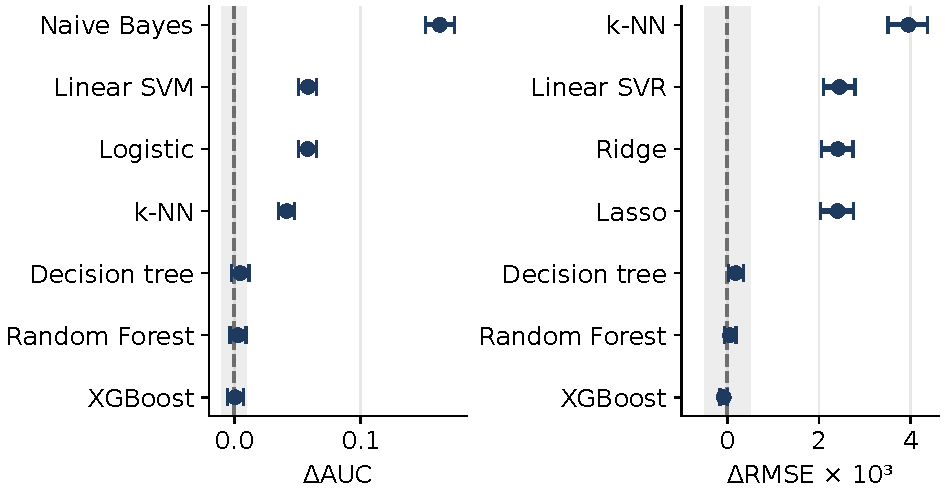
\includegraphics[width=\linewidth]{fig_intervals.pdf}
  \caption{Diferencia de la métrica principal entre la EBM y cada modelo de referencia en la prueba, con su
  intervalo \emph{bootstrap} BCa al 95~\% (2.000 réplicas): AUC (izquierda; positivo favorece a la EBM) y RMSE
  en milésimas (derecha; positivo favorece a la EBM). La banda gris es la región de equivalencia práctica.}
  \label{fig:intervals}
\end{figure}

\subsection{Resultados del estudio de ablación}
\label{sec:ablacion_res}

La tabla~\ref{tab:ablacion} y la figura~\ref{fig:ablation} comparan, con el mismo protocolo y Holm dentro de
cada tarea, las variantes que cambian el modelo con el modelo completo (ponderación, Grid, $K = 0$); la
fidelidad y la semilla no cambian el modelo y se resumen en la tabla~\ref{tab:semillas}.

\begin{enumerate}
  \item \textbf{Sin interacciones.} Como la búsqueda eligió $K = 0$, la variante se evalúa en la EBM de la
        comparación con la entrega anterior (5 pares), que sin pares obtiene 0,7185 de AUC frente a 0,7187
        (DeLong $p = 0{,}91$) y aun así supera a la logística en $+0{,}035$ ($p < 10^{-21}$). Hipótesis
        confirmada: la aditividad basta.
  \item \textbf{Balanceo.} Sin balanceo el AUC de prueba es idéntico (0,8289; probabilidad de equivalencia
        1,0); SMOTE y ADASYN lo bajan en 0,003
        sin significancia ($p$ ajustado 0,55 y 0,70) y multiplican el tiempo de la corrida por 4,4
        y 5,4. Lo que mueve el balanceo es el \emph{recall} con umbral
        0,5: 0,707 con ponderación frente a 0,355 sin ella y 0,34--0,35 con sobremuestreo. Hipótesis
        confirmada: el balanceo elige el punto de operación.
  \item \textbf{Fidelidad de la búsqueda.} En las ocho configuraciones aleatorias, la correlación de Spearman
        entre el AUC con $B = 2$ y con $B = 8$ es 0,83, la ganadora es la misma y la fidelidad
        baja ahorra el 66~\% del tiempo de búsqueda. Hipótesis confirmada.
  \item \textbf{Optimizador.} TPE y la genética llegan, con configuraciones distintas, al mismo AUC que Grid
        ($+0{,}0003$); Random Search queda $0{,}0049$ por debajo en la prueba, sin sobrevivir a Holm
        ($p = 0{,}13$) ni aparecer en los pliegues ($p = 0{,}78$). En regresión los cuatro son equivalentes. En
        las 140 corridas de la guía (tabla~\ref{tab:optimizadores_res}), Friedman rechaza por la métrica final en
        clasificación ($p = 0{,}001$, por Random Search) y no en regresión ($p = 0{,}82$); por el área de
        arrepentimiento la bayesiana tiene el menor rango en las dos tareas (Friedman $p < 10^{-6}$). Hipótesis
        confirmada en su segunda parte (la eficiencia por evaluación distingue a los métodos) y solo en parte en
        la primera: la métrica final no distingue a TPE, Grid y la genética, pero sí a Random Search en
        clasificación.
  \item \textbf{Semilla.} Con cinco semillas, la desviación del AUC de prueba de la EBM es 0,00004 y la del
        RMSE 0,000003 (tabla~\ref{tab:semillas}), de 10 a 100 veces menores que sus diferencias con los modelos
        de árboles. Hipótesis refutada para la EBM, más estable que Random Forest (0,0010) y XGBoost (0,0003),
        para los que sí se sostiene.
\end{enumerate}

\begin{table}[tbp]
  \centering\scriptsize\setlength{\tabcolsep}{1.5pt}
  \caption{Ablación: cada variante cambia un componente de la EBM completa y conserva el resto. Métrica externa (AUC o RMSE; media $\pm$ desviación de los 5 pliegues) y de prueba, \emph{recall} de prueba con umbral 0,5 (clasificación); $\Delta$ entre la variante y el modelo completo en la prueba, orientada para que un valor positivo indique que la variante pierde (AUC$_{\mathrm{comp}} -$ AUC$_{\mathrm{var}}$; en regresión RMSE$_{\mathrm{var}} - $RMSE$_{\mathrm{comp}}$ en milésimas), con intervalo BCa; $p$ de la $t$ corregida sobre los pliegues y de DeLong o Diebold-Mariano sobre la prueba, ajustados por Holm dentro de cada tarea ($^{*}$: comparación única, sin ajustar); probabilidad bayesiana de equivalencia (ROPE) entre la variante y el modelo completo. La variante sin interacciones se evalúa en la partición y la etiqueta de la comparación con la entrega anterior, donde la búsqueda sí eligió pares.}
  \label{tab:ablacion}
  \begin{tabular}{@{}>{\raggedright\arraybackslash}p{0.26\linewidth} c c c c c c c@{}}
    \toprule
    Variante & Métrica externa & Prueba & Recall$_{0{,}5}$ & $\Delta$ [IC 95~\%] & $p$ $t$ corr. & $p$ prueba & $P$(ROPE) \\
    \midrule
    EBM completa (ponderación, Grid, $K=0$) & $0{,}8292$ $\pm$ $0{,}0037$ & $0{,}8289$ & $0{,}707$ & -- & -- & -- & -- \\
    balanceo: sin balanceo (Grid) & $0{,}8285$ $\pm$ $0{,}0035$ & $0{,}8289$ & $0{,}355$ & $0{,}0000$ [$-0{,}0006$; $0{,}0006$] & $0{,}511$ & $1{,}000$ & $1{,}000$ \\
    balanceo: SMOTE (Grid) & $0{,}8278$ $\pm$ $0{,}0032$ & $0{,}8258$ & $0{,}346$ & $+0{,}0031$ [$-0{,}0008$; $0{,}0069$] & $0{,}511$ & $0{,}549$ & $1{,}000$ \\
    balanceo: ADASYN (Grid) & $0{,}8280$ $\pm$ $0{,}0033$ & $0{,}8263$ & $0{,}336$ & $+0{,}0026$ [$-0{,}0012$; $0{,}0064$] & $0{,}496$ & $0{,}702$ & $1{,}000$ \\
    optimizador: Random (ponderación) & $0{,}8276$ $\pm$ $0{,}0024$ & $0{,}8240$ & $0{,}950$ & $+0{,}0049$ [$0{,}0007$; $0{,}0092$] & $0{,}783$ & $0{,}125$ & $0{,}998$ \\
    optimizador: TPE (ponderación) & $0{,}8287$ $\pm$ $0{,}0041$ & $0{,}8286$ & $0{,}715$ & $+0{,}0003$ [$-0{,}0004$; $0{,}0010$] & $0{,}783$ & $1{,}000$ & $1{,}000$ \\
    optimizador: Genética (ponderación) & $0{,}8281$ $\pm$ $0{,}0036$ & $0{,}8287$ & $0{,}712$ & $+0{,}0003$ [$-0{,}0004$; $0{,}0009$] & $0{,}783$ & $1{,}000$ & $1{,}000$ \\
    sin interacciones ($K=0$) frente a la EBM con 5 pares (TPE) & -- & $0{,}7185$ & -- & $+0{,}0002$ [$-0{,}0029$; $0{,}0030$] & -- & $0{,}910$$^{*}$ & -- \\
    \midrule
    EBM completa (Grid, $K=0$) & $0{,}0590$ $\pm$ $0{,}0004$ & $0{,}0593$ & -- & -- & -- & -- & -- \\
    optimizador: Random & $0{,}0591$ $\pm$ $0{,}0004$ & $0{,}0592$ & -- & $-0{,}01$ [$-0{,}05$; $0{,}04$] & $0{,}581$ & $1{,}000$ & $1{,}000$ \\
    optimizador: TPE & $0{,}0590$ $\pm$ $0{,}0004$ & $0{,}0593$ & -- & $+0{,}03$ [$-0{,}02$; $0{,}09$] & $0{,}581$ & $0{,}884$ & $1{,}000$ \\
    optimizador: Genética & $0{,}0591$ $\pm$ $0{,}0004$ & $0{,}0593$ & -- & $+0{,}01$ [$-0{,}03$; $0{,}06$] & $0{,}581$ & $1{,}000$ & $1{,}000$ \\
    \bottomrule
  \end{tabular}
\end{table}

\begin{table}[tbp]
  \centering\scriptsize\setlength{\tabcolsep}{3pt}
  \caption{Sensibilidad a la semilla: modelos finales reentrenados con distintas semillas (los datos no cambian) y búsqueda del árbol de decisión repetida con cinco semillas de cada optimizador estocástico; media y desviación de la métrica de prueba.}
  \label{tab:semillas}
  \begin{tabular}{@{}l l r l c c@{}}
    \toprule
    Tarea & Modelo & Semillas & Métrica & Media & Desviación \\
    \midrule
    Clasificación & EBM (propuesto) & 5 & AUC & $0{,}8288$ & $0{,}00004$ \\
    Clasificación & Random Forest & 5 & AUC & $0{,}8281$ & $0{,}00101$ \\
    Clasificación & SVM lineal & 10 & AUC & $0{,}7706$ & $0{,}00000$ \\
    Clasificación & XGBoost & 10 & AUC & $0{,}8282$ & $0{,}00029$ \\
    Regresión & EBM (propuesto) & 5 & RMSE & $0{,}0593$ & $0{,}000003$ \\
    Regresión & Random Forest & 5 & RMSE & $0{,}0593$ & $0{,}000009$ \\
    Regresión & XGBoost & 10 & RMSE & $0{,}0592$ & $0{,}000006$ \\
    Clasificación & Árbol, búsqueda con TPE & 5 & AUC & $0{,}8246$ & $0{,}00221$ \\
    Clasificación & Árbol, búsqueda con Genética & 5 & AUC & $0{,}8243$ & $0{,}00087$ \\
    Clasificación & Árbol, búsqueda con Random & 5 & AUC & $0{,}8252$ & $0{,}00254$ \\
    \bottomrule
  \end{tabular}
  \par\smallskip\begin{minipage}{0.97\linewidth}\scriptsize Multi-fidelidad de la EBM: 8 configuraciones aleatorias evaluadas con $B=2$ y $B=8$; $\rho$ de Spearman entre los dos AUC $0{,}833$, misma configuración ganadora (sí), ahorro de tiempo de búsqueda $66$~\%.\end{minipage}
\end{table}

\begin{table}[tbp]
  \centering\small\setlength{\tabcolsep}{3pt}
  \caption{Los cuatro optimizadores con el mismo presupuesto, en los bloques modelo $\times$ balanceo con las cuatro búsquedas completas de las 140 corridas de la guía (27 en clasificación, 7 en regresión; las de la EBM se excluyen): rango medio por la métrica externa (1 = mejor), bloques ganados, segundos por evaluación, área media bajo la curva de arrepentimiento normalizado (menor es mejor) y evaluaciones hasta cerrar el 95~\% de la brecha, estas dos últimas tal como las publicó el Entregable 3.}
  \label{tab:optimizadores_res}
  \begin{tabular}{@{}l l r r r r r@{}}
    \toprule
    Tarea & Método & Rango & Victorias & s/eval. & Área arrep. & Evals.\ 95~\% \\
    \midrule
    Clas. & Grid & $2{,}22$ & 12 & $2{,}61$ & $0{,}234$ & $14{,}2$ \\
    Clas. & Random & $3{,}22$ & 4 & $2{,}46$ & $0{,}171$ & $7{,}2$ \\
    Clas. & TPE & $2{,}63$ & 2 & $4{,}48$ & $0{,}123$ & $10{,}3$ \\
    Clas. & Genética & $1{,}93$ & 15 & $4{,}27$ & $0{,}137$ & $13{,}1$ \\
    \midrule
    Regr. & Grid & $2{,}71$ & 2 & $2{,}43$ & $0{,}181$ & $9{,}9$ \\
    Regr. & Random & $2{,}71$ & 0 & $2{,}05$ & $0{,}041$ & $7{,}4$ \\
    Regr. & TPE & $2{,}14$ & 2 & $2{,}94$ & $0{,}038$ & $5{,}5$ \\
    Regr. & Genética & $2{,}43$ & 3 & $3{,}37$ & $0{,}057$ & $7{,}4$ \\
    \bottomrule
  \end{tabular}
\end{table}


\begin{figure}[tbp]
  \centering
  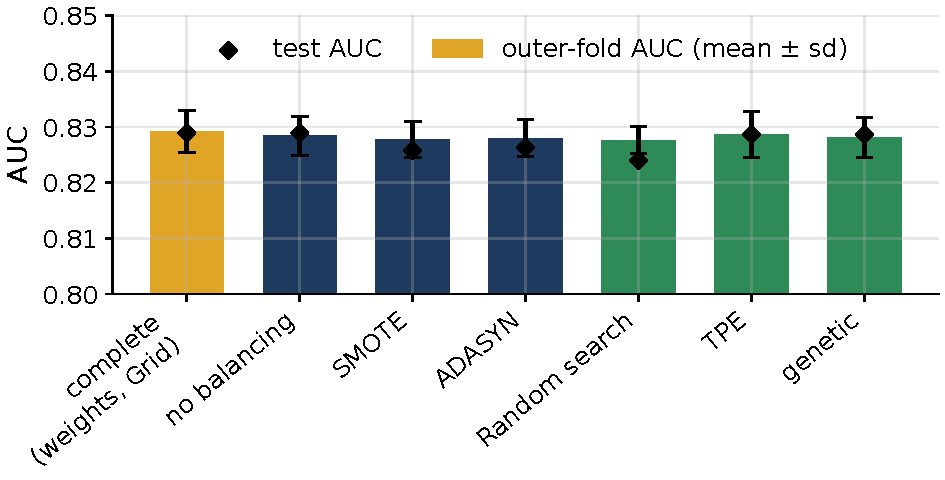
\includegraphics[width=\linewidth]{fig_ablation.pdf}
  \caption{Ablación en clasificación: AUC externa (media $\pm$ desviación de los 5 pliegues; barras) y AUC de
  prueba (rombos) del modelo completo y de cada variante de balanceo (azul) y de optimizador (verde).}
  \label{fig:ablation}
\end{figure}

\subsection{Sensibilidad y robustez}
\label{sec:sensibilidad}

La tabla~\ref{tab:semillas} y las figuras~\ref{fig:sensitivity} y~\ref{fig:hyper} reúnen las fuentes de
variabilidad. La semilla del modelo apenas pesa; la del optimizador pesa más: repetir la
búsqueda del árbol con cinco semillas mueve el AUC de prueba en 0,0009 a 0,0025, el orden de las diferencias
entre optimizadores. La sensibilidad a los hiperparámetros es baja: variando uno a la vez desde la configuración final, con validación cruzada de 3 pliegues y $B = 2$, el
AUC se mueve entre 0,8267 y 0,8292 (figura~\ref{fig:hyper}); el más influyente es el número de interacciones.
Las 16 corridas de clasificación de la EBM terminan con configuraciones muy distintas
(figura~\ref{fig:sensitivity}) y un AUC externo entre 0,8276 y 0,8292, un rango menor que la desviación entre
pliegues. La curva de aprendizaje,
ajustada con el modelo final sobre subconjuntos del entrenamiento y evaluada en la prueba, sube de 0,8234 con
2.500 clientes a 0,8288 con 38.978, y desde 10.000 solo gana 0,0018: con 2.500 clientes la EBM ya supera a la
logística entrenada con todos (0,771), mientras que el árbol es el más dependiente del tamaño; las curvas de
referencia provienen del experimento de escalamiento del Entregable 3, fuera del
pipeline anidado, por lo que Random Forest termina 0,003 por encima de su modelo final. La robustez al
desbalance se midió con y sin remuestreo (ablación): el AUC no cambia. La validación anidada predice la
prueba casi sin sesgo: en las 124 corridas de clasificación la correlación entre el AUC externo y el de
prueba es 0,997 y la diferencia media $+0{,}0016$.

\begin{figure}[tbp]
  \centering
  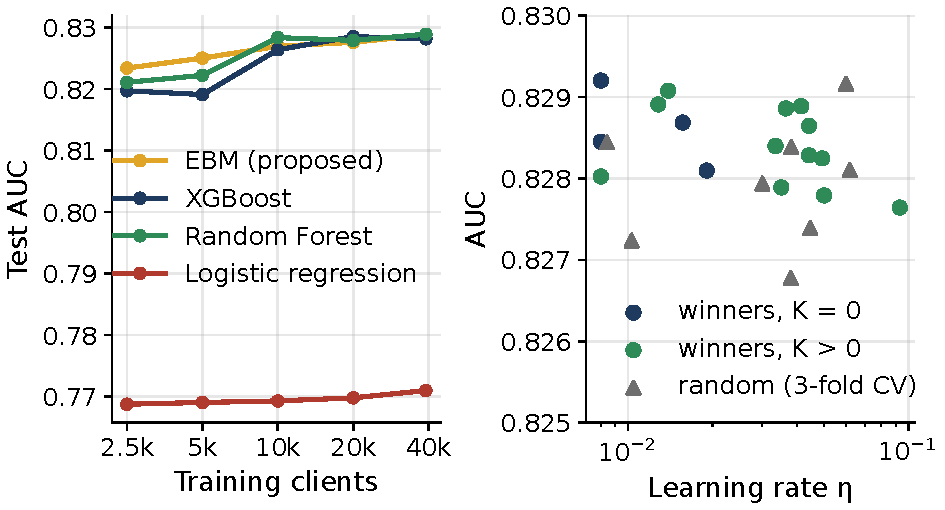
\includegraphics[width=\linewidth]{fig_sensitivity.pdf}
  \caption{Izquierda: curva de aprendizaje (AUC de prueba frente al número de clientes de entrenamiento, con
  los hiperparámetros finales de cada modelo; la EBM se ajusta en el guion de esta sección y las referencias
  provienen del experimento de escalamiento del Entregable 3). Derecha: AUC de la EBM frente a la tasa de
  aprendizaje en las 16 configuraciones ganadoras de las corridas (círculos; azul $K = 0$, verde $K > 0$; AUC
  externo) y en las ocho configuraciones aleatorias de la prueba de fidelidad (triángulos; validación cruzada de
  3 pliegues con $B = 8$).}
  \label{fig:sensitivity}
\end{figure}

\begin{figure}[tbp]
  \centering
  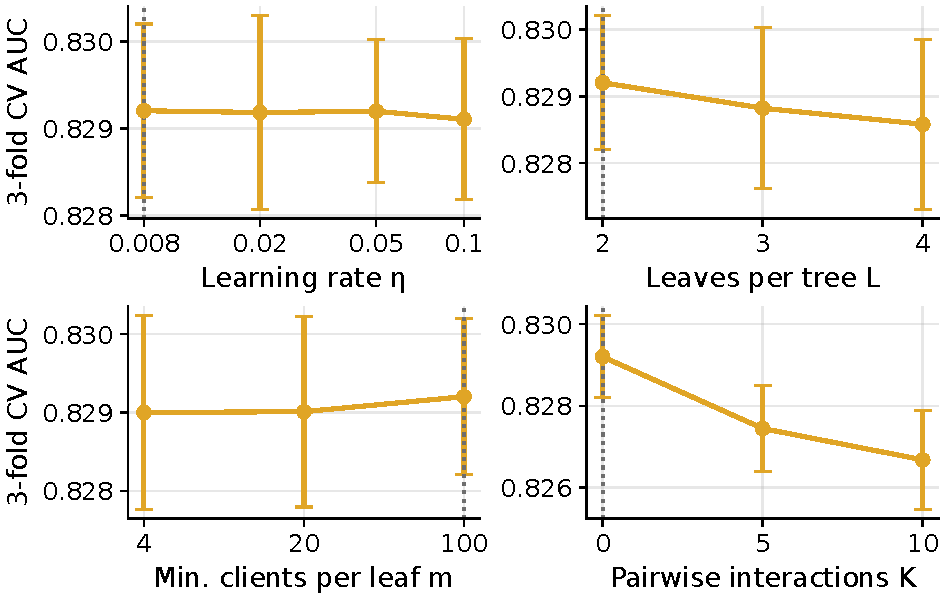
\includegraphics[width=\linewidth]{fig_hyper.pdf}
  \caption{Sensibilidad de la EBM a cada hiperparámetro por separado: AUC (media $\pm$ desviación de una
  validación cruzada de 3 pliegues sobre el entrenamiento, con $B = 2$) al variar la tasa de aprendizaje, las
  hojas por árbol, el mínimo de clientes por hoja y el número de interacciones desde la configuración final
  (línea punteada).}
  \label{fig:hyper}
\end{figure}

\subsection{Costo computacional}
\label{sec:costo}

Según la tabla~\ref{tab:costo}, la EBM es el modelo más lento de ajustar: 26,7~s en clasificación y 31,8~s en
regresión, 17 y 15 veces más que XGBoost (1,6 y 2,1~s) y del orden de Random Forest. En inferencia está en el
grupo rápido (0,067~s para los 9.745 clientes, tres veces menos que Random Forest y cien menos que k-NN),
ocupa 1,5~MB frente a 44~MB del bosque, guarda 15.485 valores frente a 574.556 nodos y
necesita 20~MB de memoria pico en el ajuste frente a 68~MB del bosque. La EBM no mejora el AUC de XGBoost y
cuesta 17 veces más en ajuste, pero el ajuste ocurre una vez y la consulta es igual de barata; el costo extra
compra un modelo legible sin explicador.

\begin{table}[tbp]
  \centering\scriptsize\setlength{\tabcolsep}{3pt}
  \caption{Costo computacional de la mejor combinación de cada modelo en el equipo de referencia (AMD de 6 núcleos, 15,9~GB): ajuste del modelo final sobre los 38.978 clientes y puntuación de los 9.745 de prueba (mediana de 3 y 5 repeticiones con el pipeline completo), duración de la corrida anidada completa, tamaño serializado, número de parámetros (valores almacenados: nodos de los árboles, puntajes de las funciones de forma, coeficientes; k-NN guarda la matriz de entrenamiento) y memoria pico del ajuste por encima de la base: en clasificación la midió el Entregable 3 (la de la EBM se midió aquí, mediana de tres ajustes) y en regresión se midió aquí para todos.}
  \label{tab:costo}
  \begin{tabular}{@{}l l r r r r r r@{}}
    \toprule
    Tarea & Modelo & Ajuste (s) & Inferencia (s) & Corrida (min) & Tamaño (MB) & Parámetros & Memoria (MB) \\
    \midrule
    Clas. & k-NN & $0{,}28$ & $7{,}164$ & $34{,}7$ & $23{,}50$ & 3.040.284 & $<1$ \\
    Clas. & Naive Bayes & $0{,}30$ & $0{,}068$ & $0{,}7$ & $0{,}01$ & 314 & $24$ \\
    Clas. & SVM lineal & $0{,}92$ & $0{,}052$ & $2{,}1$ & $<0{,}01$ & 79 & $32$ \\
    Clas. & Árbol de decisión & $1{,}38$ & $0{,}054$ & $1{,}8$ & $0{,}01$ & 53 & $12$ \\
    Clas. & XGBoost & $1{,}61$ & $0{,}060$ & $8{,}9$ & $0{,}56$ & 14.063 & $13$ \\
    Clas. & Regresión logística & $1{,}83$ & $0{,}056$ & $3{,}1$ & $<0{,}01$ & 79 & $61$ \\
    Clas. & Random Forest & $23{,}65$ & $0{,}187$ & $20{,}9$ & $43{,}97$ & 574.556 & $68$ \\
    Clas. & \textbf{EBM (propuesto)} & $26{,}72$ & $0{,}067$ & $18{,}7$ & $1{,}49$ & 15.485 & $20$ \\
    \midrule
    Regr. & k-NN & $0{,}25$ & $4{,}725$ & $24{,}9$ & $23{,}50$ & 3.040.284 & $<1$ \\
    Regr. & Ridge & $0{,}28$ & $0{,}046$ & $1{,}5$ & $<0{,}01$ & 79 & $24$ \\
    Regr. & Lasso & $0{,}46$ & $0{,}046$ & $6{,}7$ & $<0{,}01$ & 79 & $23$ \\
    Regr. & SVR lineal & $0{,}66$ & $0{,}046$ & $2{,}7$ & $<0{,}01$ & 79 & $29$ \\
    Regr. & Árbol de decisión & $0{,}84$ & $0{,}047$ & $3{,}7$ & $0{,}01$ & 71 & $12$ \\
    Regr. & XGBoost & $2{,}09$ & $0{,}065$ & $10{,}4$ & $0{,}46$ & 3.582 & $5$ \\
    Regr. & Random Forest & $12{,}31$ & $0{,}145$ & $16{,}1$ & $6{,}01$ & 85.948 & $13$ \\
    Regr. & \textbf{EBM (propuesto)} & $31{,}85$ & $0{,}054$ & $26{,}6$ & $1{,}49$ & 15.485 & $25$ \\
    \bottomrule
  \end{tabular}
\end{table}


\subsection{Interpretabilidad y análisis de errores}
\label{sec:errores}

\paragraph{Qué usa el modelo.}
La tabla~\ref{tab:importancia} ordena los términos de la EBM de clasificación: la edad (37,8~\%), la
frecuencia de uso de la aplicación (30,1~\%), la satisfacción (11,6~\%) y la satisfacción de base (2,5~\%)
reúnen el 82~\% de la importancia, y la importancia por permutación en la prueba coincide (caídas de AUC de
0,177 a 0,0008; ningún otro predictor llega a 0,0003). Son las cuatro variables del
análisis exploratorio y las que SHAP \citep{lundberg2017shap} señala en XGBoost en el Entregable 3. Las
funciones de forma (figura~\ref{fig:shapes}) muestran la no linealidad que los modelos lineales no captan: la
edad no es monótona (de $-1{,}57$ a $+1{,}40$ en el logit), la frecuencia de uso reduce el riesgo con fuerza
hasta unos 20 inicios de sesión y luego se aplana, la satisfacción actúa por escalones y la de base sigue una
curva en S.

\paragraph{Dónde falla.}
La tabla~\ref{tab:errores} divide la prueba por cohorte de edad y por \ap, la variable excluida. La cohorte de
59--60 años, con el 46~\% de riesgo alto, es la más difícil (AUC 0,645 dentro de la cohorte); la de 44--45
(9~\%) la más fácil (0,922). La EBM y XGBoost alcanzan el mismo \emph{recall} global con clientes distintos:
con la capacidad del 25~\%, la EBM contacta sobre todo a la cohorte mayor (deja fuera al 37~\% de sus
clientes de riesgo alto, pero al 91~\% de los de 44--45) y XGBoost reparte más (56~\% y 34~\%), porque la edad domina al modelo aditivo; de los
1.171 clientes de riesgo alto que la EBM deja fuera, 563 son de 59--60 años, 354 de 29--30 y 254 de 44--45.
Por \ap, en cambio, el AUC dentro de cada nivel está entre 0,988 y 0,999 en los dos modelos y el sesgo de la
regresión forma una escalera: $-0{,}055$ con un producto, $-0{,}005$ con dos, $+0{,}045$, $+0{,}095$ y
$+0{,}145$ con tres, cuatro y cinco. El modelo pronostica a todos cerca del nivel de dos productos porque no
ve cuántos tienen; los errores grandes son la parte del objetivo que depende de la variable excluida y explican
la compresión y la asimetría de la figura~\ref{fig:regression}. La tabla~\ref{tab:ejemplos} muestra tres
clientes representativos de esos errores; en los dos primeros la edad y el uso de la aplicación apuntan en
sentido contrario al nivel de \ap, que decide el puntaje real.

\begin{table}[tbp]
  \centering\small\setlength{\tabcolsep}{3pt}
  \caption{Interpretabilidad de la EBM de clasificación: cuota de la importancia de cada término (media del valor absoluto de su función de forma sobre el entrenamiento; los 78 términos suman 100~\%) e importancia por permutación sobre la prueba (caída media $\pm$ desviación del AUC al permutar cada predictor original, 5 repeticiones).}
  \label{tab:importancia}
  \begin{tabular}{@{}l r l c@{}}
    \toprule
    Término (EBM) & Cuota & Predictor permutado & Caída del AUC \\
    \midrule
    \texttt{age} & $37{,}8$~\% & \texttt{age} & $0{,}1772$ $\pm$ $0{,}0050$ \\
    \texttt{app\_logins\_frequency} & $30{,}1$~\% & \texttt{app\_logins\_frequency} & $0{,}1159$ $\pm$ $0{,}0062$ \\
    \texttt{satisfaction\_score} & $11{,}6$~\% & \texttt{satisfaction\_score} & $0{,}0282$ $\pm$ $0{,}0021$ \\
    \texttt{base\_satisfaction} & $2{,}5$~\% & \texttt{base\_satisfaction} & $0{,}0008$ $\pm$ $0{,}0005$ \\
    \texttt{income\_bracket\_Low} & $1{,}5$~\% & \texttt{prop\_Transfer} & $0{,}0002$ $\pm$ $0{,}0001$ \\
    \texttt{prop\_Withdrawal} & $1{,}0$~\% & \texttt{customer\_tenure} & $0{,}0002$ $\pm$ $0{,}0001$ \\
    \texttt{product\_satisfaction} & $0{,}9$~\% & \texttt{credit\_utilization\_ratio} & $0{,}0001$ $\pm$ $0{,}0001$ \\
    \texttt{investment\_account} & $0{,}8$~\% & \texttt{investment\_account} & $0{,}0001$ $\pm$ $0{,}0000$ \\
    \bottomrule
  \end{tabular}
\end{table}

\begin{table}[tbp]
  \centering\scriptsize\setlength{\tabcolsep}{2pt}
  \caption{Análisis de errores en la prueba por cohorte de edad y por número de productos activos (variable excluida del modelo): tamaño, prevalencia de riesgo alto, AUC de la EBM y de XGBoost dentro del segmento, fracción de clientes de riesgo alto que cada modelo deja fuera del 25~\% contactado (FN, falsos negativos), RMSE de regresión de los dos modelos y sesgo medio del pronóstico de la EBM (pronóstico $-$ real).}
  \label{tab:errores}
  \begin{tabular}{@{}l r r c c c c c c c@{}}
    \toprule
    Segmento & $n$ & Prev. & AUC EBM & AUC XGB & FN EBM & FN XGB & RMSE EBM & RMSE XGB & Sesgo EBM \\
    \midrule
    cohorte de edad 29--30 & 3.224 & $18$~\% & $0{,}830$ & $0{,}840$ & $60$~\% & $38$~\% & $0{,}0598$ & $0{,}0598$ & $+0{,}001$ \\
    cohorte de edad 44--45 & 3.174 & $9$~\% & $0{,}922$ & $0{,}930$ & $91$~\% & $34$~\% & $0{,}0586$ & $0{,}0584$ & $0{,}000$ \\
    cohorte de edad 59--60 & 3.347 & $46$~\% & $0{,}645$ & $0{,}636$ & $37$~\% & $56$~\% & $0{,}0594$ & $0{,}0593$ & $0{,}000$ \\
    \midrule
    productos activos 1 & 3.918 & $54$~\% & $0{,}997$ & $0{,}999$ & $55$~\% & $55$~\% & $0{,}0548$ & $0{,}0548$ & $-0{,}055$ \\
    productos activos 2 & 2.939 & $9$~\% & $0{,}996$ & $0{,}995$ & $0$~\% & $0$~\% & $0{,}0067$ & $0{,}0057$ & $-0{,}005$ \\
    productos activos 3 & 1.390 & $0$~\% & $0{,}999$ & $0{,}988$ & $0$~\% & $0$~\% & $0{,}0456$ & $0{,}0453$ & $+0{,}045$ \\
    productos activos 4 & 1.016 & $0$~\% & -- & -- & -- & -- & $0{,}0954$ & $0{,}0953$ & $+0{,}095$ \\
    productos activos 5 & 482 & $0$~\% & -- & -- & -- & -- & $0{,}1453$ & $0{,}1453$ & $+0{,}145$ \\
    \bottomrule
  \end{tabular}
\end{table}

\begin{table}[tbp]
  \centering\scriptsize\setlength{\tabcolsep}{3pt}
  \caption{Tres clientes de prueba representativos de los errores: el de riesgo alto con menor puntaje de la EBM (FN, el falso negativo más grave), el de riesgo bajo con mayor puntaje (FP, el falso positivo más grave) y el de mayor error absoluto de regresión, con sus variables de señal, el nivel de \ap\ (que el modelo no ve), su puntaje real y las predicciones de la EBM y de XGBoost.}
  \label{tab:ejemplos}
  \begin{tabular}{@{}l c c c@{}}
    \toprule
    Variable & FN más grave & FP más grave & Mayor error de regresión \\
    \midrule
    Edad (años) & 44 & 60 & 44 \\
    Inicios de sesión & $22$ & $4$ & $37$ \\
    Satisfacción & $3$ & $3$ & $4$ \\
    \ap & 1 & 4 & 5 \\
    Riesgo alto real & sí & no & no \\
    Puntaje real & $0{,}393$ & $0{,}351$ & $0{,}153$ \\
    Prob. EBM / XGBoost & $0{,}206$ / $0{,}590$ & $0{,}988$ / $0{,}648$ & $0{,}075$ / $0{,}315$ \\
    Pron. EBM / XGBoost & $0{,}334$ / $0{,}341$ & $0{,}442$ / $0{,}440$ & $0{,}311$ / $0{,}305$ \\
    \bottomrule
  \end{tabular}
\end{table}


\begin{figure}[tbp]
  \centering
  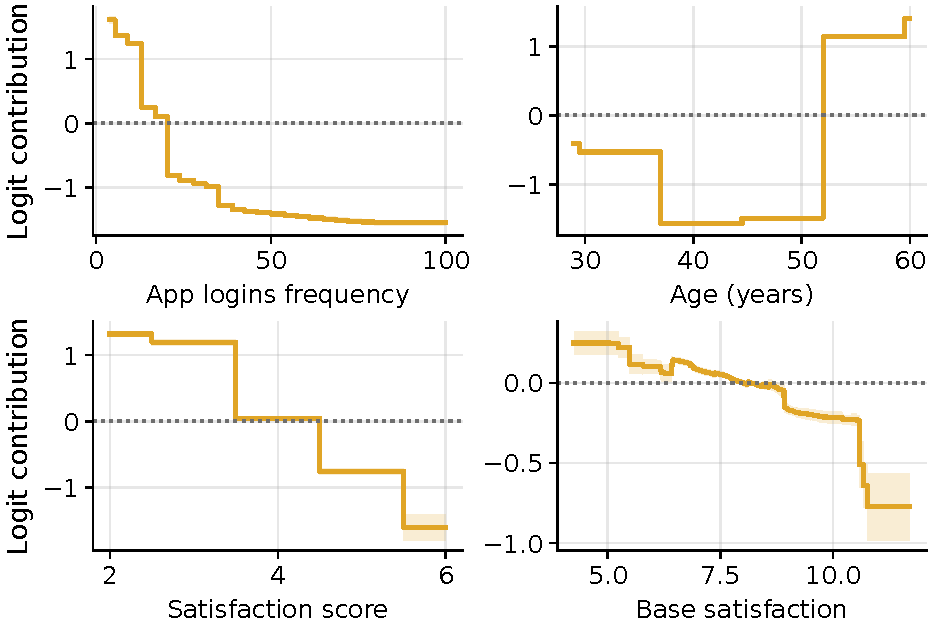
\includegraphics[width=\linewidth]{fig_shapes.pdf}
  \caption{Funciones de forma de la EBM de clasificación para las cuatro variables con señal: contribución al
  logit del riesgo alto (centrada) con la banda entre las 8 bolsas externas, en las unidades originales de cada
  variable.}
  \label{fig:shapes}
\end{figure}

\subsection{Discusión, limitaciones y amenazas a la validez}
\label{sec:discusion}

Los resultados sugieren que, en este problema, un modelo aditivo con funciones de forma alcanza la misma
capacidad predictiva que los ensambles de árboles: la EBM empata con XGBoost, Random Forest y el árbol en las
dos tareas y supera con claridad a los modelos lineales, a k-NN y a Naive Bayes, como en \citet{lou2013ga2m}.
La ablación explica por qué aquí ni siquiera hacen
falta las interacciones: la señal está en cuatro variables con efectos no lineales y casi independientes, de
modo que lo que faltaba en la entrega anterior era flexibilidad por variable, no profundidad. El empate con
XGBoost es una propiedad de los datos: el techo de información sin \ap\ estimado en el Entregable 3 es 0,7223
de AUC (etiqueta de la mediana) y 0,2197 de $R^2$, y la EBM cubre el 98~\% de ambos ($\auc - 0{,}5$).

Hay un solo conjunto de datos, con rasgos sintéticos (cohortes de edad, escalera de productos activos), y el
objetivo es el puntaje de otro modelo, no la fuga observada. Con cinco pliegues la $t$ corregida tiene 4 grados de libertad y poca potencia, y McNemar en el punto
de operación es insensible a diferencias que el AUC sí ve. Otras amenazas son menores: el SVM es lineal (el núcleo RBF multiplicaba por
70 el costo), la logística cubre L1 y L2 como un solo modelo, la regresión no incluye un modelo bayesiano, los
tiempos son de un solo equipo y, aunque las variables derivadas no usan el objetivo, en un conjunto sintético
no puede descartarse una fuga residual. La conclusión proporcional a la evidencia es que la EBM es una
alternativa equivalente a XGBoost en precisión, más lenta de ajustar, igual de rápida en inferencia y legible
por construcción; no que sea mejor.
